\subsection{Number of expected Neutrinos based on NuGen Datasets}
The simulation uses nugen datasets to calculate the number of expected
neutrinos according to the standard formula (cite ???).
\begin{equation}
\label{eq:Nexp_general}
 N_\text{exp}^\nu = \sum_i\frac{dF_P(E_i)}{dE_i} \cdot
\frac{OneWeight_i}{N_\text{generated}}
\end{equation}
The nugen simulation describes the probability for each simulated neutrino event
$i$ to reach the detector,
interact within its effective volume and to be detected ($OneWeight_i$), the
individual energy $E_i$ and the number of generated MC neutrino events
$N_\text{generated}$.

%  and a re-weighting factor $\frac{A_{ZB}}{4 \pi}$. The
% re-weighting factor will be explained in more detail in section ???. 
The differential particle fluence $\frac{dF_P}{dE}$ at earth needs to be
calculated based on the GRB properties drawn at source - peak luminosity
$\hat{L}_\text{Peak}$, $\hat{t}_{90, S}$, redshift (sections \ref{sec:Etotal} -
\ref{sec:FatEarth}). Values at source are marked with a
hat while values on earth are represented by the appropriate characters 
themselves.


\subsubsection{Zenith Bands}
\label{sec:zenith_bands}
The probability to detect a neutrino is highly dependent on the zenith angle of
its origin. The number of expected neutrinos within IceCube can be
calculated for all simulated events (eq. \ref{eq:Nexp_general}). However, these
are distributed over the whole sky and might not represent a GRB from a
specific zenith direction very well. Therefore, only events from a zenith 
region around
a drawn GRB direction will be used to calculate the expected signal. The true
direction of each considered event needs to be within a range around the GRB
direction in $\text{Cos} \Theta$
\begin{equation}
\text{Cos}\left(\Theta_{\nu, \text{true}}\right) \in
\left[\text{Cos}\left(\Theta_\text{GRB}\right) - ZBW,\,
\text{Cos}\left(\Theta_\text{GRB}\right) +
ZBW\right]
\end{equation}
The zenith band width is set to $ZBW = 0.05$ and equal in cosinus of the zenith
angle to achieve similar (and enough) statistics near pole and horizon. 

%??? above horizon?

%A side effect might be that more deviation towards pole 
Consequently, the number of expected neutrino events within the detector (eq.
\ref{eq:Nexp_general}) is not calculated anymore based on the total number of
generated events $N_\text{generated}$ over the whole sky but only a fraction of
events within the zenith band. Therefore, $N_\text{generated}$ needs to be
replaced by an effective number of generated events
\begin{equation}
N_\text{generated}^\text{eff} = N_\text{generated} \cdot \frac{A_{ZB}}{4\pi}
\end{equation}
in which $A_{ZB}$ is the area of the zenith band. The number of expected
neutrinos is then 
\begin{equation}
\label{eq:Nexp_wZB}
 N_\text{exp}^\nu = \sum_i\frac{dF_P(E_i)}{dE_i} \cdot
\frac{OneWeight_i}{N_\text{generated}^\text{eff}} = 
\sum_i\frac{dF_P(E_i)}{dE_i} \cdot
\frac{OneWeight_i}{N_\text{generated} \cdot \frac{A_{ZB}}{4\pi}}
\end{equation}
\subsection{Shifting Event Positions to GRB position}
\label{sec:shift2source}
In later steps the directions of different neutrino events will be compared to
each other. Therefore, all events within a zenith band need to be shifted such
that their true
direction $\vec{t}$ will coincide with the GRB direction $\vec{g}$ and the
shifted or new reconstructed direction $\vec{n}$ should have the same distance
and direction
to $\vec{g}$ as the originally reconstructed direction $\vec{r}$ had to
$\vec{t}$.

The following calculations will be made in cartesian coordinates by
transforming the zenith and azimuth angle
\begin{equation}
 \begin{align}
  x &= \text{sin}\theta \cdot \text{cos} \phi \\
  y &= \text{sin}\theta \cdot \text{sin} \phi \\
  z &= \text{cos}\theta\\
 \end{align}
\end{equation}
with $\phi \in [0, 2 \pi)$, $\theta \in [0, \pi]$
The angular difference between $\vec{t}$ and $\vec{r}$ is
\begin{equation}
 \text{cos} \alpha = \frac{\vec{r} \cdot \vec{t}}{|\vec{r}| |\vec{t}|}
\end{equation}
and the direction of $\vec{r}$ relative to $\vec{t}$ is
\begin{equation}
 \vec{e} = \frac{\vec{r} - \vec{t}}{|\vec{r} - \vec{t}|}
\end{equation}
Therefore, the following conditions need to be met
\begin{align}
 \text{cos} \alpha &= \frac{\vec{r} \cdot \vec{t}}{|\vec{r}| |\vec{t}|} =
\frac{\vec{n} \cdot \vec{g}}{|\vec{n}| |\vec{g}|} \\
\vec{n} & = \vec{g} + c \vec{e}
\end{align}
leaving the factor c to be the only unkown to determine $\vec{n}$. There should
be two solutions, one in the positive and one in the negative direction
yealding two possible vectors that fullfill the same angular distance to the GRB
direction $\vec{g}$. As $\vec{e}$ points into the intended direction, $c$ will
be always chosen as positive.

Combining the conditions, one can derive the factor $c$
\begin{equation}
\label{eq:ang_dist_shifting}
 \begin{align}
 \text{cos} \alpha &= \frac{\vec{n} \cdot \vec{g}}{|\vec{n}| |\vec{g}|} \\
&= \frac{\left(\vec{g} + c \vec{e} \right) \cdot \vec{g}}{|\vec{g} + c
\vec{e}| |\vec{g}|} \\
&= \frac{\left(g_x + c \cdot e_x\right) \cdot g_x + \left(g_y + c \cdot
e_y\right) \cdot g_y + \left(g_z + c \cdot e_z\right) \cdot
g_z}{\sqrt{\left(g_x + c e_x \right)^2 + \left(g_y + c e_y \right)^2 +\left(g_z
+ c e_z \right)^2 } \cdot \sqrt{g_x^2 + g_y^2 +g_z^2}} \\
&= \frac{g_x^2 + g_y^2 +g_z^2 + c \cdot \left(e_x g_x + e_y g_y + e_z g_z
\right)}{\sqrt{g_x^2 + g_y^2 +g_z^2 + 2 c \cdot \left(e_x g_x + e_y g_y + e_z
g_z \right) + c^2 \left( e_x^2 + e_y^2 + e_z^2 \right) } \cdot \sqrt{g_x^2 +
g_y^2 +g_z^2}} \\
&= \frac{\gamma + c \cdot \tau}{\sqrt{\gamma + 2 c \cdot \tau + c^2 \cdot \zeta}
\sqrt{\gamma}}
 \end{align}
\end{equation}
with the abbreviations
\begin{equation}
 \begin{align}
  \gamma &= \vec{g}^2 = g_x^2 + g_y^2 +g_z^2 \\
  \tau &= \vec{g}\cdot \vec{e}=e_x g_x + e_y g_y + e_z g_z\\
  \zeta &=  \vec{e}^2 =e_x^2 + e_y^2 + e_z^2
 \end{align}
\end{equation}
Calculating the square of equation \ref{eq:ang_dist_shifting} and rewriting it
to fit the
standard p,q - formulism, one obtains
\begin{equation}
 \begin{align}
\left(
\gamma + 2 c \cdot \tau + c^2 \cdot \zeta \right) \gamma \cdot \text{cos}^2
\alpha - \left(\gamma^2 + 2 c \tau \gamma  + c^2 \tau^2 \right) &= 0\\
\text{cos}^2\alpha \left(\gamma^2 + 2 c \cdot \tau \gamma + c^2 \cdot \zeta
\gamma \right) - \left( \gamma^2 + 2 c \tau \gamma  + c^2 \tau^2\right) &= 0\\
c^2 \cdot \left(\zeta \gamma \text{cos}^2\alpha - \tau^2 \right) + 2 c \cdot
\tau \gamma \left( \text{cos}^2\alpha - 1 \right) + \gamma^2 \left(
\text{cos}^2\alpha - 1 \right)  &= 0 \\
c^2 + c \cdot \frac{ 2 \tau \gamma \left(\text{cos}^2\alpha - 1 \right)}{\zeta
\gamma \text{cos}^2\alpha - \tau^2} + \frac{\gamma^2 \left(
\text{cos}^2\alpha - 1 \right) }{\zeta
\gamma \text{cos}^2\alpha - \tau^2} &= 0 \\
c^2 + p \cdot c + q &= 0
%  \end{align}
%  \begin{align}
 \end{align}
\end{equation}
Therefore, $c$ has two solutions as predicted. The positive will always be
chosen.
\begin{equation}
 c = -  \frac{\tau \gamma \left(\text{cos}^2\alpha - 1 \right)}{\zeta
\gamma \text{cos}^2\alpha - \tau^2} \pm \sqrt{\left( \frac{\tau \gamma
\left(\text{cos}^2\alpha - 1 \right)}{\zeta
\gamma \text{cos}^2\alpha - \tau^2} \right)^2 - \frac{\gamma^2 \left(
\text{cos}^2\alpha - 1 \right) }{\zeta
\gamma \text{cos}^2\alpha - \tau^2}}
\end{equation}

The value of c leads to the calculation of the new reconstructed direction
$\vec{n}$ which can be transformed back into spherical coordinates using
\begin{equation}
 \theta = \text{arccos} \left( \frac{n_z}{|\vec{n}|} \right)
\end{equation}
\begin{equation}
 \begin{align}
  \phi &= \text{arctan} \left( \frac{n_y}{n_x}\right)  \text{,  if  } n_x > 0\\
  \phi &= sign \left(n_y \right) \cdot \frac{\pi}{2}  \text{,  if  } n_x = 0\\
  \phi &= \text{arctan} \left( \frac{n_y}{n_x}\right) + \pi  \text{,  if  } n_x
<0 \text{ and } n_y \geq 0\\
  \phi &= \text{arctan} \left( \frac{n_y}{n_x}\right) - \pi  \text{,  else}\\
 \end{align}
\end{equation}


% \begin{framed}
% There are very few events for which this is
% not true. The reason is unknown at this moment. 
% \end{framed}
 


 
\begin{figure}[htbp]
  \centering
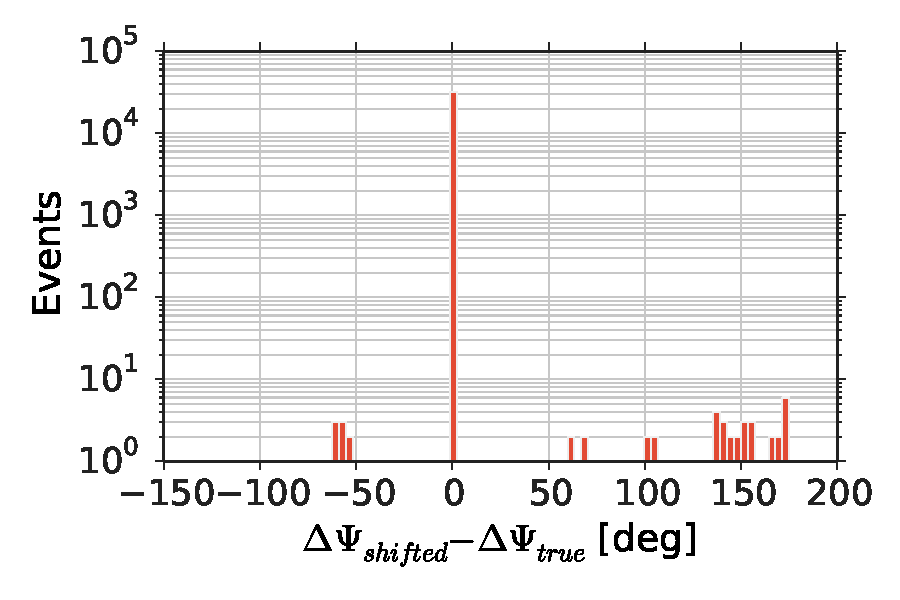
\includegraphics[width=
1.\textwidth]{fig/shift2source_true_minus_shifted_error.pdf}
  \caption{\label{fig:shift2source_proof}Shown is the difference between the
true error between reconstructed and true direction and the error between the
shifted reconstructed direction and the GRB direction. Almost all events have 
been shifted perfectly.}
\end{figure}

\begin{figure}[h]
\centering
 \captionsetup{width=.9\textwidth}
%  \captionsetup{margin=0pt}
\subfloat[Dependency on zenith angle.\label{fig:shift2source_zendependency}]{%
 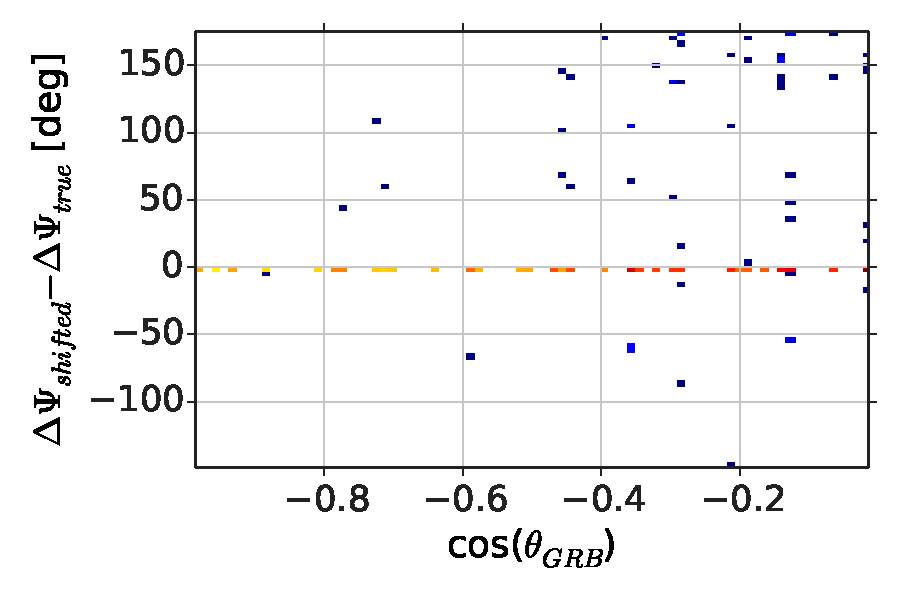
\includegraphics[width=0.45\textwidth]{fig/shift2source_zendependency.pdf}}
 \subfloat[Dependency on the azimuth angle. 
\label{fig:shift2source_azidependency}]{%
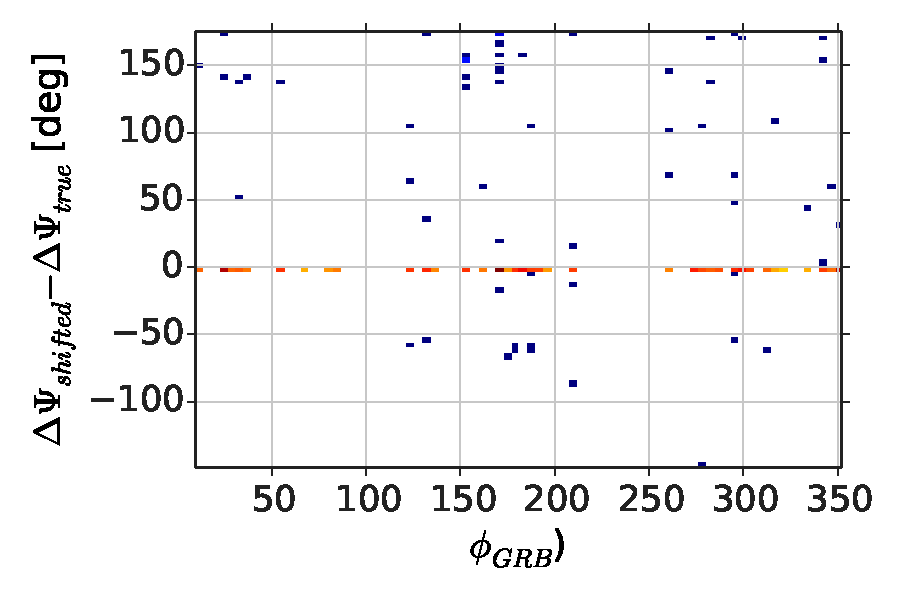
\includegraphics[width=0.45\textwidth]{fig/shift2source_azidependency.pdf}}
\caption{Two dimensional histograms showing the dependency of the difference 
between shifted and true reconstruction error to the zenith (left) and azimuth 
angle (right). No true dependency can be seen.}
\end{figure}

Figure \ref{fig:shift2source_proof} demonstrates that, for almost all events, 
the new directions 
have
 the same distance to the GRB as the originally
reconstructed directions had compared to their true directions. There are few 
events \textbf{(I need a percentage here!!!???)} for which the process doesn't 
work. The reasons are unknown at this point. Figures 
\ref{fig:shift2source_zendependency} and \ref{fig:shift2source_azidependency} 
demonstrate that there is no directional correlation. However, as this effect 
is only true for ???\% of the events, the effect can be neglected.
% An example skymap for one GRB and the correspondingly shifted neutrino
% directions is shown in Figure \ref{fig:skymap_grb}.




\subsubsection{Total Emitted Energy as Source $\hat{E}_{\nu, \text{total}}$}
\label{sec:Etotal}
So far, the steps dealing with simulation effects and neutrino directions have
been described. To calculate $N_\text{exp}^\nu$ the differential particle
fluence in energy at earth needs to be calculated as well, based on parameters
that are drawn as part of the simulation (chapter \ref{sec:drawnProp}). A first
step is to calculate the total emitted energy in neutrinos at the source
$\hat{E}_{\nu, \text{total}}$.

The peak luminosity and the 90\% time window can be used if the light curve is
known. In
this work a fast rise and rapid decay (FRED) light curve with an instant jump
to the peak luminosity and an exponential decay afterwards is assumed. 

%comment about test if this is folded into normalization?

The luminosity at a given time $\hat{t}$ is defined as 
\begin{equation}
 \hat{L}(\hat{t}) = \hat{L}_{\text{Peak}} \cdot e^{\left(-
\frac{\hat{t}}{\hat{\tau}}\right)}
\label{eq:lum_vs_time}
\end{equation}
The total energy is the time integral over the time dependent luminosity
distribution
\begin{equation}
\label{eq:Eiso}
\begin{align}
 \hat{E}_{\nu, \text{total}} & =  \int_0^{\infty} \hat{L}(\hat{t}) d\hat{t} 
	  =  \hat{L}_{\text{Peak}} \int_0^{\infty} e^{-\frac{t}{\tau}} dt\\
	 & = - \hat{\tau} \cdot \hat{L}_{\text{Peak}} \left[
e^{-\frac{\hat{t}}{\hat{\tau}}}
\right]_0^{\infty}
          = \hat{\tau} \cdot \hat{L}_{\text{Peak}}
\end{align}
\end{equation}
The final shape of the distribution depends on the unknown $\tau$ which needs to
be replaced by a known quantity such as the 90 \% time window
$\hat{t}_{90}$ in which 90\% or $\hat{E}_{\nu, 90}=0.9 \cdot \hat{E}_{\nu,
\text{total}}$ are
observed. 
The amount of energy radiated within this time can be determined with
\begin{equation}
 \begin{align}
  \hat{E}_{\nu, 90} & = 0.9 \cdot \hat{E}_{\nu, \text{total}} = 0.9 \cdot
\hat{\tau} \hat{L}_{\text{Peak}} = 
\int_0^{\hat{t}_{90}} \hat{L}(\hat{t}) d\hat{t} \\
         & = - \hat{\tau} \hat{L}_{\text{Peak}}
\left[e^{-\frac{\hat{t}}{\hat{\tau}}} \right]_0^{\hat{t}_{90}}
= \hat{\tau} \hat{L}_{\text{Peak}} \left[1 -
e^{-\frac{\hat{t}_{90}}{\hat{\tau}}} \right]
 \end{align}
\end{equation}
leading to 
\begin{equation}
 \begin{align}
  \left[ 1 - e^{-\frac{\hat{t}_{90}}{\hat{\tau}}} \right] &= 0.9 \\
 0.1 & = e^{-\frac{\hat{t}_{90}}{\hat{\tau}}} \\
 \text{ln}(0.1) & = -\frac{\hat{t}_{90}}{\hat{\tau}}\\
 \Rightarrow \hat{\tau} &= \frac{-\hat{t}_{90}}{\text{ln}(0.1)}
 \label{eq:ToyMC_tau}
 \end{align}
\end{equation}
Entering this in equation \ref{eq:Eiso} leads to:
\begin{equation}
 \hat{E}_{\nu, \text{total}} = - \hat{L}_{\text{Peak}}
\frac{\hat{t}_{90}}{\text{ln}(0.1)}
\end{equation}


\subsubsection{Fluence at Source}
The simulation draws GRB properties at source. In the first step they are used
to calculate the differential particle fluence in energy
$\frac{d\hat{F}_P}{d\hat{E}}$ in units $\text{GeV}^{-1}
\text{s}^{-1}\text{sr}^{-1} \text{cm}^{-2}$ at a small co-moving distance from
the source $\hat{d}_0$. The spectral shape is a generalization based on the fits
to the HESE flux (eq. \ref{eq:HESEflux_gen}).

\begin{equation}
 \frac{d\hat{F}_P}{d\hat{E}} = \frac{\hat{F}_0}{4 \pi \hat{d}_0^2} \cdot
\hat{E}^{-\gamma} \text{exp} \left( - \frac{\hat{E}}{\hat{E}_\text{cut}} \right)
\end{equation}
The fluence normalization $\hat{F}_0$ is unknown. However, in the previous
section \ref{sec:Etotal} the total emitted energy was calculated. It equals the
integral over $\hat{E} \cdot \frac{d\hat{F}_P}{d\hat{E}}$.

\begin{equation}
\label{eq:Etotal}
 \hat{E}_{\nu, \text{total}} = \int_{\hat{E}_{min}}^\infty \hat{E} \hat{F}_0
\hat{E}^{-\gamma} \text{exp} \left(  -
\frac{\hat{E}}{\hat{E}_\text{cut}}\right) d\hat{E} = \hat{F}_0
\Upsilon \left(\hat{E}_{min}, \hat{E}_\text{cut}\right)
\end{equation}
The result depends on two GRB parameters which are chosen equally as physics 
parameters
for all GRBs: A minimal energy of the neutrinos $\hat{E}_{min}$ and the
break energy $\hat{E}_{cut}$. Once, these parameters are chosen, $\Upsilon$ is
a constant for all GRBs and the differential particle fluence in energy at
source can be written as

\begin{equation}
 \frac{d\hat{F}_P}{d\hat{E}} = \frac{\hat{E}_{\nu, \text{total}}}{4 \pi
d_0^2\Upsilon\left(\hat{E}_{min}, \hat{E}_\text{cut}\right)} \cdot
\hat{E}^{-\gamma}
\text{exp} \left( - \frac{\hat{E}}{\hat{E}_\text{cut}} \right)
\label{eq:partFluenceS}
\end{equation}
%  The impact 

\subsubsection{Fluence at Earth}
\label{sec:FatEarth}
Having derived the fluence at source, cosmological effects need to be taken
into account when calculating the fluence at earth. The energy and time
at source relate to the values at earth with $\hat{E} = (1 + z) E$ and 
$\hat{t} = \frac{t}{1+z}$. 
The energy flux at earth $\Phi_E$ is linked to the luminosity via
\begin{equation}
\label{eq:PhiEL}
 \Phi_E (t) = \frac{\hat{L} \left(\hat{E}, \hat{t} \right)}{4 \pi d_l^2} =
\frac{L \left(E, t \right)}{4 \pi d_l^2}
\end{equation}
with the luminosity distance $d_l=(1+z) \cdot d_c$.
The particle fluence $F_P$ at earth is the time integrated particle flux
$\Phi_P$ which in turn is the energy derivative of the energy flux.
\begin{equation}
F_P(E) = \int \Phi_P(E,t)\, dt = \int
\frac{d\Phi_E(E,t)}{dE}\,dt 
% = \frac{dN(E)}{dA}
\label{eqn:fluence}
\end{equation}

% \begin{equation}
% \Phi_E (t) = \int \Phi_P(E,t) \, dE = \int \frac {dN(E,t)}{dA\,dt}\, dE.
% \label{eqn:fluxes}
% \end{equation}
% \begin{eqnarray}
%   \frac {dN(E,t)}{dA\,dt} = \Phi_P =  \frac{d\Phi_E(E,t)}{dE}
%    & = & \frac{1}{4 \pi d_l^2} \frac {d L(t)}{dE}
% \end{eqnarray}
% \begin{eqnarray}
% \frac {dF_P(E)}{dE} = \frac {dN(E)}{dA\,dE} & = &  \int \frac{\Phi_P(E,t)}{dE}\,
% dt %\\
% %   & = & \frac{1}{4 \pi d_l^2} \int \frac{d^2 L(t)}{dE^2} dt
%   \label{eqn:local}
% \end{eqnarray}
The energy flux can be replaced with the luminosity according to
\ref{eq:PhiEL}. Applying a derivation in energy and transforming energy and
time to the source frame, one obtains
\begin{eqnarray}
  \frac {dF_P(E)}{dE}
     & = &  \frac{1}{4 \pi d_l^2} \int \frac{d^2 L(t)}{dE^2} dt \\
     & = &  \frac{1}{4 \pi d_l^2} \int \frac{d^2 L(\hat{t})}{d\hat{E}^2}
     \frac{d^2\hat{E}}{dE^2} \frac{dt}{d\hat{t}}
     d\hat{t} \\
     & = & \frac{(1+z)^3} {4 \pi d_l^2} \int \frac{d^2 L(\hat{t})}{d\hat{E}^2}
     d\hat{t}
     \label{eqn:final}
\end{eqnarray}
A similar equation is true for differential particle fluence in energy near the
source at a distance $d_0$.
\begin{eqnarray}
\frac {d\hat{F}_P(\hat{E})}{d\hat{E}}
  & = & \frac{1}{4 \pi d_0^2} \int \frac{d^2 L(\hat{t})}{d\hat{E}^2} d\hat{t}
  \label{eqn:grb}
\end{eqnarray}
Combining equation \ref{eqn:final} and \ref{eqn:grb} relates the differential
particle fluence at earth to the differential particle fluence at source
derived in \ref{eq:partFluenceS}.
\begin{eqnarray}
  \frac{dF_P(E)}{dE}
    & = & \left(\frac{d_0}{d_l}\right)^2 (1+z)^3 \frac
{d\hat{F}_P(\hat{E})}{d\hat{E}} \\
&=& \frac{\hat{E}_{\nu, \text{total}}}{4 \pi
d_l^2\Upsilon\left(\hat{E}_{min}, \hat{E}_\text{cut}\right)} \cdot
\hat{E}^{-\gamma}
\text{exp} \left( - \frac{\hat{E}}{\hat{E}_\text{cut}} \right) \cdot (1+z)^3 \\
&=& \frac{\hat{E}_{\nu, \text{total}}}{4 \pi
d_l^2\Upsilon\left(\hat{E}_{min}, \hat{E}_\text{cut}\right)} \cdot
E^{-\gamma}
\text{exp} \left( - \frac{E \cdot (1+z)}{\hat{E}_\text{cut}} \right) \cdot
(1+z)^{3 - \gamma}
\end{eqnarray}
In the last step the energy at source was replaced with the energy at earth in
consideration of the cosmological effects. This formula can now be used to
calculate the number of expected neutrinos within IceCube given the drawn
properties and a nugen dataset (section \ref{subsubsec:NExp}).

\subsubsection{Number of Expected Neutrinos Within IceCube}
\label{subsubsec:NExp}
This chapter described how the differential particle fluence in energy can be
derived from the drawn parameters describing a GRB in this simulation. The
number of expected neutrinos is  given with

%??? detail about  nugen and oneweight. cite paper on oneweight. detector
% response

\begin{equation}
\begin{align}
 N_\text{exp}^\nu & = \sum_i\frac{dF_P(E_i)}{dE} \cdot
\frac{OneWeight_i}{N_\text{generated} \cdot A_{ZB}} \\
&= \sum_i \cdot \frac{\hat{E}_{\nu, \text{total}}}{4 \pi
d_l^2\Upsilon\left(\hat{E}_{min}, \hat{E}_\text{cut}\right)} \cdot
E_i^{-\gamma}
\text{exp} \left( - \frac{E_i \cdot (1+z)}{\hat{E}_\text{cut}} \right) \cdot
(1+z)^{3 - \gamma}
\frac{OneWeight_i}{N_\text{generated} \cdot \frac{A_{ZB}}{4 \pi}}
\end{align}
\end{equation}
It is dependent on various factors of the nugen simulation and some parameters
from the derivation of the differential particle fluence. The nugen simulation
describes the probability for each simulated event $i$ to reach the detector,
interact within its effective volume and to be detected ($OneWeight_i$), the
individual energy $E_i$, the number of generated MC neutrino events
$N_\text{generated}$ and a re-weighting factor $\frac{A_{ZB}}{4 \pi}$. The
re-weighting factor has been explained in more detail in section ???. 

Furthermore, the number of expected neutrinos is dependent on the redshift of
the GRB, the total emitted energy in neutrinos $\hat{E}_{\nu, \text{total}}$ -
and thus $\hat{L}_\text{Peak}$ and $\hat{t}_{90}$ - as well as the constant
$\Upsilon$. The constant itself is dependent on the energy of the cut-off
$\hat{E}_\text{cut}$ and the minimal neutrino energy at source $\hat{E}_{min}$.
As described in ??? the cut-off energy will be optimized to reproduce the
observed cut-off or set to very high values depending on the spectrum that is
used (see ???). The effect of the minimal energy can be either absorbed into
the normalization to the HESE flux (chapter \ref{sec:norm2HESE}) or specific
cases and their impact can be studied (chapter ???).